\documentclass[nooutcomes]{ximera}
%% handout
%% space
%% newpage
%% numbers
%% nooutcomes


\newcommand{\RR}{\mathbb R}
\renewcommand{\d}{\,d}
\newcommand{\dd}[2][]{\frac{d #1}{d #2}}
\renewcommand{\l}{\ell}
\newcommand{\ddx}{\frac{d}{dx}}
\newcommand{\dfn}{\textbf}
\newcommand{\eval}[1]{\bigg[ #1 \bigg]}

\usepackage{multicol}

\renewenvironment{freeResponse}{
\ifhandout\setbox0\vbox\bgroup\else
\begin{trivlist}\item[\hskip \labelsep\bfseries Solution:\hspace{2ex}]
\fi}
{\ifhandout\egroup\else
\end{trivlist}
\fi} %% we can turn off input when making a master document
\usepackage{fullpage}

\title{Section - 2.4:  Infinite Limits}  

\begin{document}
\begin{abstract}		\end{abstract}
\maketitle

%Problem1
\begin{problem}
  \outcome{Match graphs of functions with their equations based on vertical asymptotes.}
  Without using a graphing utility, match each graph of functions in A-F with the aglebraic representation of functions in a-f:

  \begin{center}
    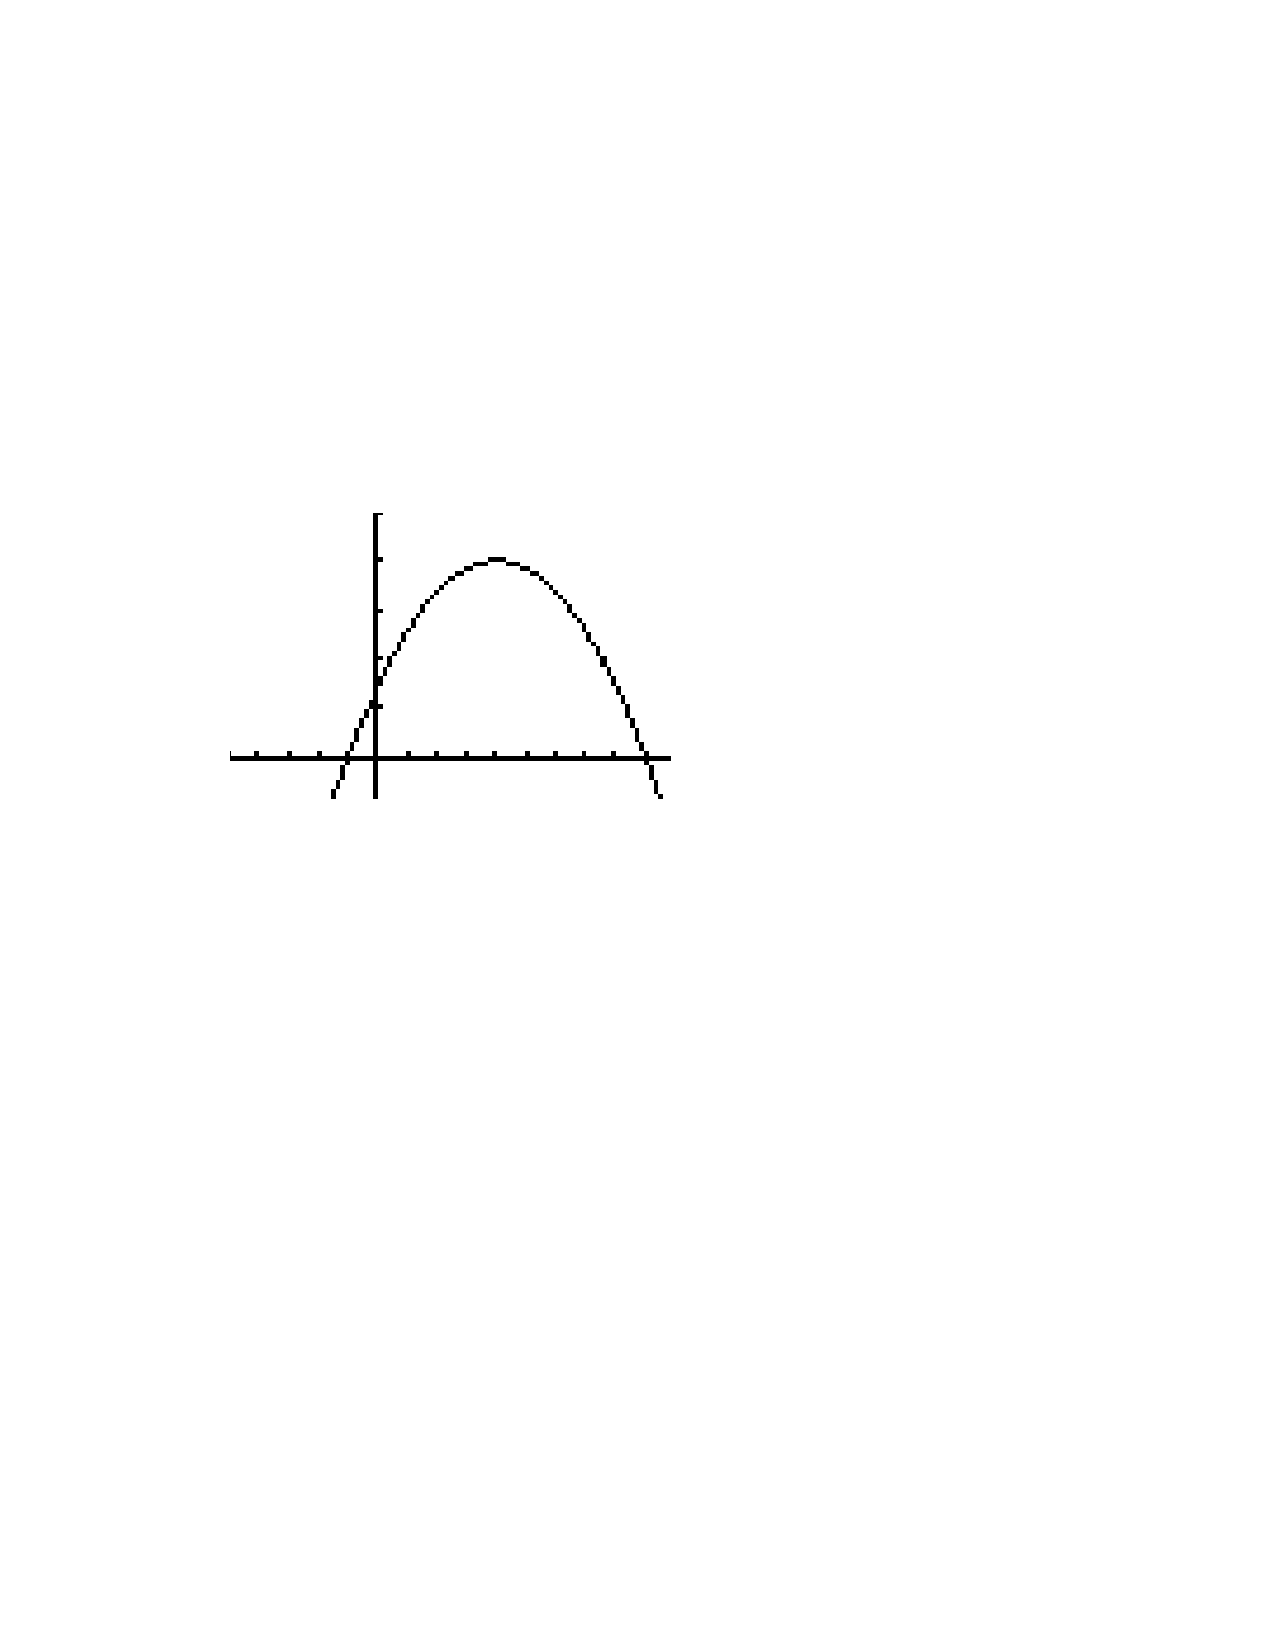
\includegraphics[trim= 250 360 300 185]{Figure1.pdf}
  \end{center}

  \begin{enumerate}
    \item
      The function $f$ defined by $\displaystyle f(x) = \frac{x}{x^2 + 1}$.

      \begin{freeResponse}
        Since there is no real number $x$ such that $x^2 + 1 = 0$, we have no candidates for vertical asymptotes.
        Hence the graph of $f$ should not contain any vertical asymptotes.
        The only listed graph with no vertical asymptote is graph D.
      \end{freeResponse}

    \item 
      The function $g$ defined by $\displaystyle g(x) = \frac{x}{x^2 -1}$.
      \begin{freeResponse}
        \emph{Candidates} for vertical asymptotes:
        \begin{align*}
          x^2 -1 = 0 &\implies \mbox{$x = 1$ or $x = -1$.}
        \end{align*}

        Test of candidate $x = 1$:
        \begin{align*}
          \lim_{x \to 1^+} \frac{x}{x^2 -1} &= \lim_{x \to 1^+}\frac{x}{(x-1)(x+1)} = \infty \\
	&\text{Because this limit is of the form:} \frac{\text{ pos}}{0^+} \\
          &\implies \mbox{vertical asymptote at $x = 1$}
        \end{align*}
        
        Test of candidate $x = -1$:
        \begin{align*}
          \lim_{x \to -1^-} \frac{x}{x^2 -1} &= \lim_{x \to -1^-} \frac{x}{(x-1)(x+1)}= -\infty \\
	&\text{Because this limit is of the form:} \frac{\text{ neg}}{0^+}\\
          &\implies \mbox{vertical asymptote at $x = -1$}
        \end{align*}

        Since $g(0) = 0$, the only listed graph that can match is graph C.
      \end{freeResponse}


    \item 
      The function $h$ defined by $\displaystyle h(x) = \frac{1}{x^2 -1}$.
      \begin{freeResponse}
        \emph{Candidates} for vertical asymptotes: $x = 1$ and $x = -1$.

        Test of candidate $x = 1$:
        \begin{align*}
          \lim_{x \to 1^+} \frac{1}{x^2 -1} &= \lim_{x \to 1^+} \frac{1}{(x-1)(x+1)} = \infty\\
	&\text{Because this limit is of the form:} \frac{\text{ pos}}{0^+} \\
          &\implies \mbox{vertical asymptote at $x = 1$}.
        \end{align*}

        Test of candidate $x = -1$:
        \begin{align*}
          \lim_{x \to -1^-} \frac{1}{x^2 -1} &= \lim_{x \to -1^-} \frac{1}{(x-1)(x+1)} = \infty\\
	&\text{Because this limit is of the form:} \frac{\text{ pos}}{0^+} \\
          &\implies \mbox{vertical asymptote at $x = -1$}.
        \end{align*}
        Since $h(0) = -1$, the only listed graph that can match is graph F.
      \end{freeResponse}

    \item 
      The function $a$ defined by $\displaystyle a(x) = \frac{x}{(x-1)^2}$.
      \begin{freeResponse}
        Candidate for the vertical asymptote: $x = 1$.

        Test of candidate $x = 1$:

        \begin{align*}
          \lim_{x \to 1^+}\frac{x}{(x-1)^2} &= \infty \\
	&\text{Because this limit is of the form:} \frac{\text{ pos}}{0^+}\\
          &\implies \mbox{vertical asymptote at $x = 1$}
        \end{align*}
        Since $a(0) = 0$ the graph is graph B.
      \end{freeResponse}

    \item 
      The function $s$ defined by $\displaystyle s(x) = \frac{1}{(x-1)^2}$.
      \begin{freeResponse}
        Candidate for the vertical asymptote: $x = 1$.

        Test of candidate $x = 1$:

        \begin{align*}
          \lim_{x \to 1^+} \frac{x}{(x-1)^2} &= \infty \\
	&\text{Because this limit is of the form:} \frac{\text{ pos}}{0^+} \\
          &\implies \mbox{vertical asymptote at $x = 1$}
        \end{align*}
        Since $s(0) = 1$ the graph is graph A.        
      \end{freeResponse}


    \item
      The function $r$ defined by $\displaystyle r(x) = \frac{x}{x+1}$.
      \begin{freeResponse}
        Candidate for the vertical asymptote: $x = -1$.

        Test of candidate $x = -1$:

        \begin{align*}
          \lim_{x \to -1^+} \frac{x}{x+1} &= -\infty \\
	&\text{Because this limit is of the form:} \frac{\text{ neg}}{0^+} \\
          &\implies \mbox{vertical asymptote at $x = -1$}
        \end{align*}
        Since $r(0) = 0$ the graph is graph E.
      \end{freeResponse}

  \end{enumerate}

\end{problem}

%Problem2
\begin{problem}
  Evaluate each of the following limits or say that the limit does not exist. Make sure to state the form of the limit.
  If a limit does not exist, explain why.

  \begin{enumerate}
	\item
      $\displaystyle \lim_{x \to 3^-} \frac{x^2 - 3}{x^2 - x - 6}$
      \begin{freeResponse} Checking right sided limit we have:


         $ \lim_{x \to 3^-} \frac{x^2 - 3}{x^2 - x - 6} = \lim_{x \to 3^-} \frac{x^2 - 3}{(x-3)(x+2)}$  is of the form:  $\frac{\text{ pos}}{0^-}$

	$$\lim_{x \to 3^-} \frac{x^2 - 3}{x^2 - x - 6} =-\infty$$
      \end{freeResponse}

    \item
      $\displaystyle \lim_{x \to 5^+} \frac{x^2 + 6}{x^2 - 3x - 10}$
      \begin{freeResponse}
       Checking left and right sided limits we have:
        \begin{align*}
          \lim_{x \to 5^+} \frac{x^2 + 6}{x^2 - 3x - 10} &= \lim_{x \to 5^+} \frac{x^2 + 6}{(x-5)(x+2)}  = \infty \\
	&\text{because the limit is of the form:} \frac{\text{ pos}}{0^+}
        \end{align*}
      \end{freeResponse}

    \item
      $\displaystyle \lim_{x \to 1} \frac{4-x}{x^2 - 2x + 1}$
      \begin{freeResponse}
        Checking left and right sided limits we see:
        \begin{align*}
          \lim_{x \to 1^+} \frac{4-x}{x^2 - 2x + 1} &= \lim_{x \to 1^+}\frac{4-x}{(x-1)^2} = \infty\\
	&\text{because the limit is of the form:} \frac{\text{ pos}}{0^+}
        \end{align*}
 	 and
        \begin{align*}
 	\lim_{x \to 1^-} \frac{4-x}{x^2 - 2x + 1} &= \lim_{x \to 1^-}\frac{4-x}{(x-1)^2} = \infty\\
	&\text{because the limit is of the form:} \frac{\text{ pos}}{0^+}
	\end{align*}
	Since $\lim_{x \to 1^-} \frac{4-x}{x^2 - 2x + 1}=\lim_{x \to 1^+} \frac{4-x}{x^2 - 2x + 1} \implies  \lim_{x \to 1} \frac{4-x}{x^2 - 2x + 1} = \infty$
      \end{freeResponse}

    \item
      $\displaystyle \lim_{x \to 2} \frac{-e^x}{(2-x)^3}$
      \begin{freeResponse}
        Checking left limit we have:
 \begin{align*}
          \lim_{x \to 2^+} \frac{-e^x}{(2-x)^3} &= \infty\\
	&\text{because the limit is of the form:} \frac{\text{neg}}{0^-}
        \end{align*}
 	 and
        \begin{align*}
 	\lim_{x \to 2^-} \frac{-e^x}{(2-x)^3} &= - \infty\\
	&\text{because the limit is of the form:} \frac{\text{neg}}{0^+}
	\end{align*}
	Since $ \lim_{x \to 2^+} \frac{-e^x}{(2-x)^3} \ne \lim_{x \to 2^-} \frac{-e^x}{(2-x)^3} \implies   \lim_{x \to 2} \frac{-e^x}{(2-x)^3}$ Does not exist
      \end{freeResponse}
\end{enumerate}
\end{problem}

%Problem3
\begin{problem}
	Sketch a possible graph of a function $g$ that satisfies the following conditions:
	\begin{align*}
	&\text{Domain:} [-5,-2) \cup (-2,3) \cup (3,5)
	& \lim_{x \to -2} g(x) = 3\\
	& g(1)=1
	& \lim_{x \to 1^+} g(x) = -\infty\\
	& \lim_{x \to 3} g(x) = \infty
	& \lim_{x \to 5^-} g(x) = \infty\\
	& \lim_{x \to 1^-} g(x) = 1
	& g(-5)=-1.8
	\end{align*}
	\begin{freeResponse}
	First we will draw our domain on the x-axis using green.  We will use a bracket when a point is in the domain and curved parenthesis when it is not.
  \begin{center}
    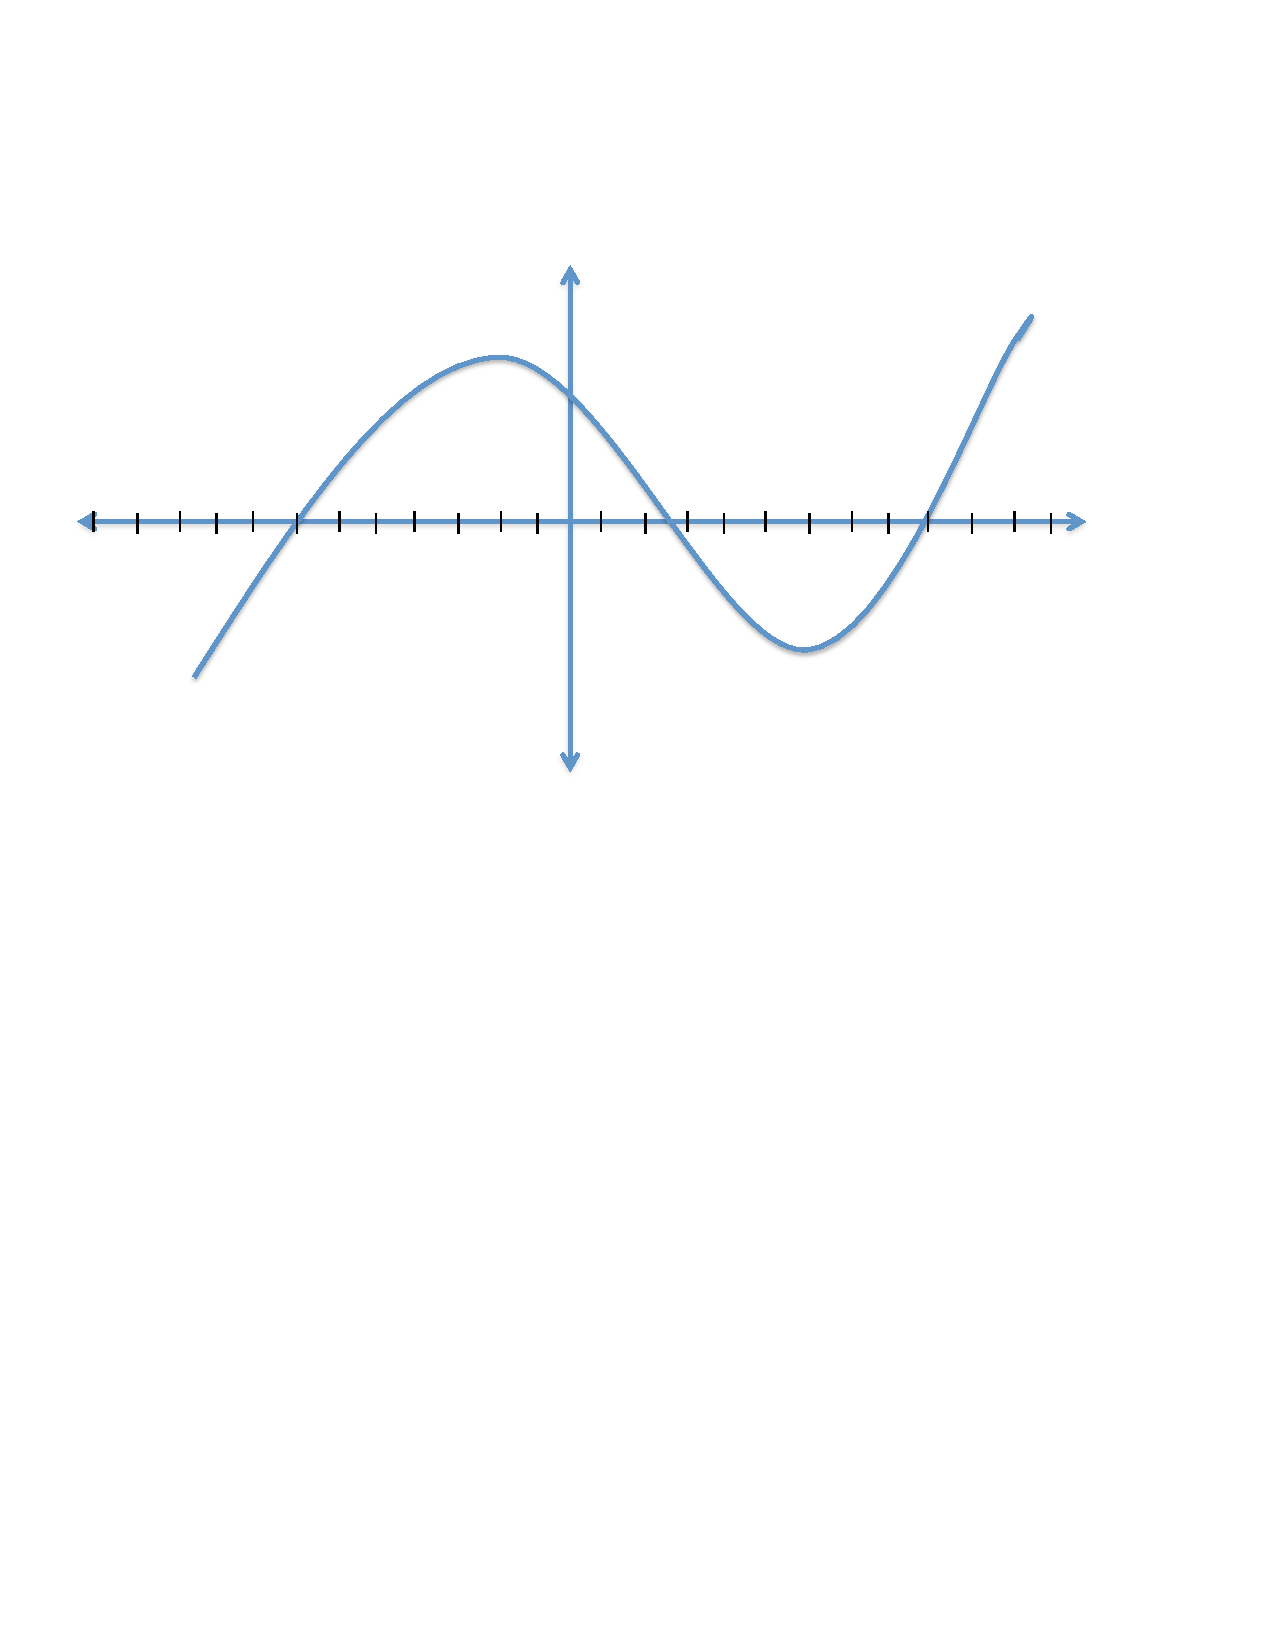
\includegraphics[scale=.5]{Figure2.pdf}
  \end{center}
	Next, we draw and open circle at $(-1,3)$ because we know $\lim_{x \to -2} g(x) = 3$.  We also draw a closed circle at (1,1) and (-5,-1.8) because we know $g(1)=1$ and $g(-5)=-1.8$.  Finally we draw in our vertical asymptotes in purple as indicated by the infinite limits at $x=1, x=3, x=5$.  We draw the tails of the asmyptotes in blue to indice whether the function $g$ approaches $ -\infty$ or $\infty$.
  \begin{center}
    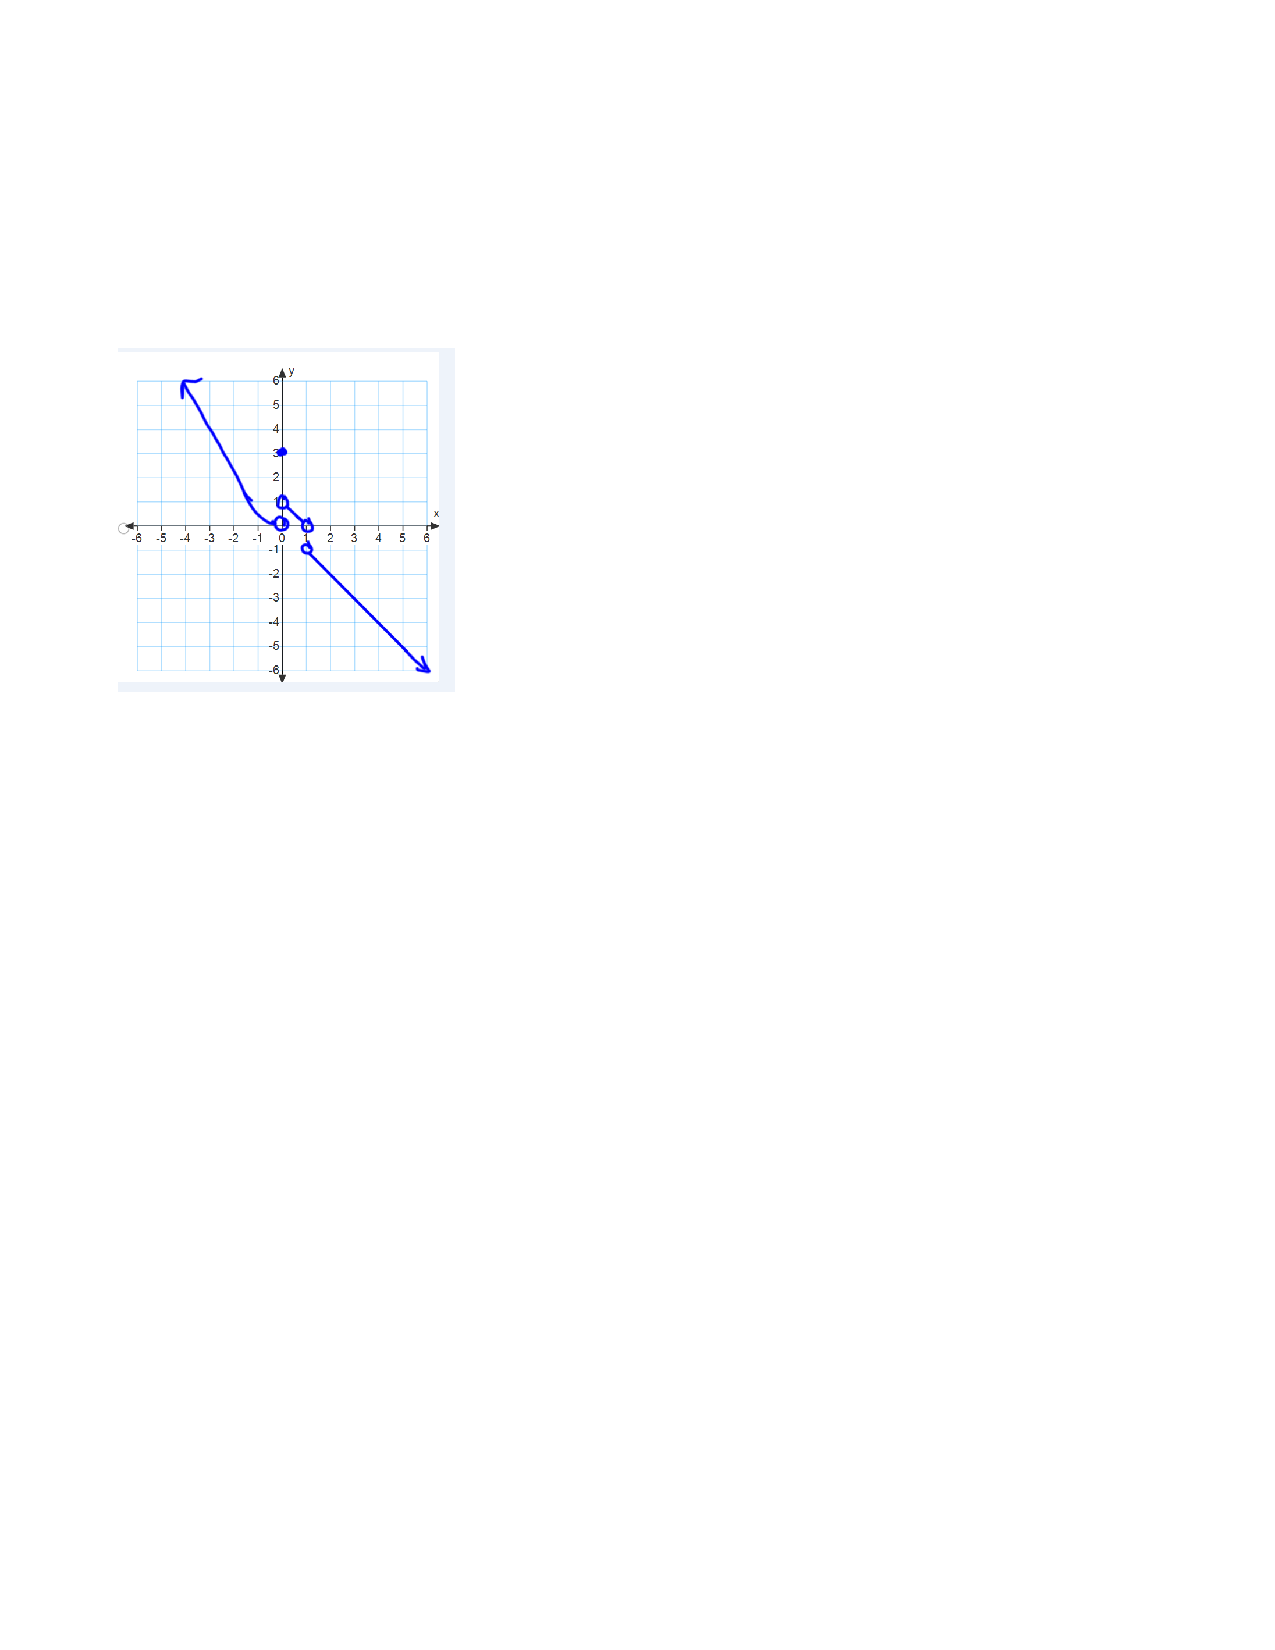
\includegraphics[scale=.5]{Figure3.pdf}
  \end{center}
	Finally, we connect our graph together.
  \begin{center}
    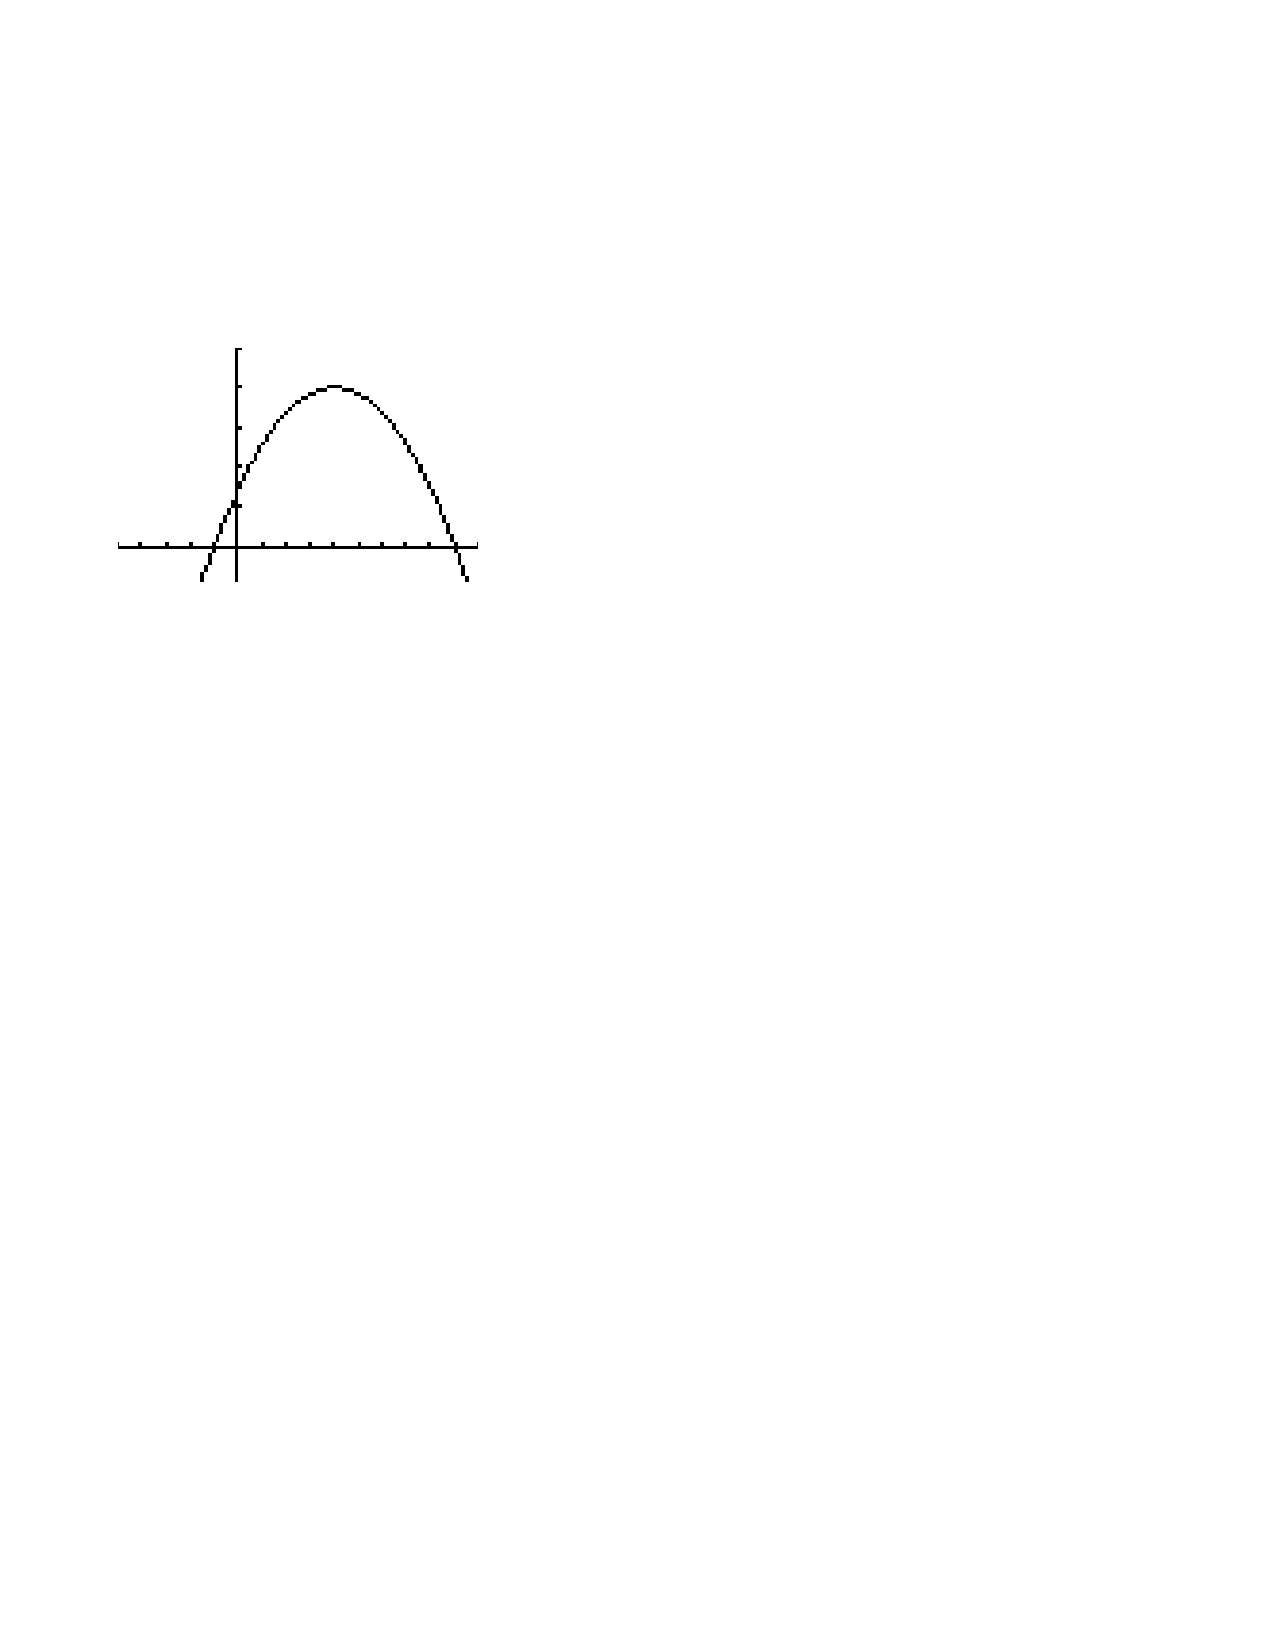
\includegraphics[scale=.5]{Figure4.pdf}
  \end{center}
	\end{freeResponse}
\end{problem}

%Problem4
\begin{problem}
	\begin{enumerate}
  \item
      $\displaystyle \lim_{x \to 3} \frac{x^2 - 2x - 3}{\sqrt{x+1} - 2}$
      \begin{freeResponse}
        We have
        \begin{align*}
          \lim_{x \to 3} \frac{x^2 - 2x - 3}{\sqrt{x+1} - 2} &= \lim_{x \to 3} \frac{(x- 3)(x + 1)}{\sqrt{x+1} - 2} \text{This is of the form $\frac{0}{0}$} \\
          &= \lim_{x \to 3} \frac{(x- 3)(x + 1)}{\sqrt{x+1} - 2} \cdot \frac{\sqrt{x+1} + 2}{\sqrt{x+1} + 2}\\
          &= \lim_{x \to 3} \frac{(x- 3)(x + 1)(\sqrt{x+1} + 2)}{x+1 - 4}\\
          &= \lim_{x \to 3} \frac{(x- 3)(x + 1)(\sqrt{x+1} + 2)}{x-3}\\
          &= \lim_{x \to 3} (x + 1)(\sqrt{x+1} + 2) = 4 \cdot 4 = 16
        \end{align*}
      \end{freeResponse}


    \item
      $\displaystyle \lim_{x \to 0^+} x \cdot \sin(\ln(x))$.
      \begin{freeResponse}
	We know sine of any number is always between $-1$ and $1$, so we have $-1 \le  \cdot \sin(\ln(x)) \le 1$.
	\begin{align*}
	(-1 \le  \cdot& \sin(\ln(x)) \le 1) \cdot x\\
       	-x \le x \cdot& \sin(\ln(x)) \le x\ \text{for}\ x \text{postive and near} 0\\
	\text{Since}\ \lim_{x \to 0^+} -x = 0,\ &\text{and}\ \lim_{x \to 0^+} x = 0\ \text{By Squeeze theorem we get:}\\
          &\lim_{x \to 0^+} x \cdot \sin(\ln(x)) = 0
 		\end{align*}
      \end{freeResponse}


    \item
      $\displaystyle \lim_{x \to 2^-} \frac{\ln(x)}{x - 2}$.
      \begin{freeResponse}
       
        \begin{align*}
        	\text{This is of the form:}\frac{\text{pos}}{0^-} \text{and thus} \lim_{x \to 2^-} \frac{\ln(x)}{x - 2} = -\infty.
        \end{align*}
      \end{freeResponse}
  \end{enumerate} 
\end{problem}


%Problem5
\begin{problem}
Let $f$ be a function given by $f(x)=\ln(1+x)$.

	\begin{enumerate}
	\item Find the domain of $f$.  Write your answer in interval notation.
	\begin{freeResponse}
	$1+x>0 \implies x>-1 \implies \text{domain:}(-1,+\infty)$
	\end{freeResponse}
	
	\item Find the vertical asymptotes of $f$ and justify.
	\begin{freeResponse}
	$g(x)=\ln(x)$ has a vertical asymptote at $x=0$.  $f$ is $g$ shifted one unit left so $f$ will have a vertical asymptote at $x=-1$. 
	
	\end{freeResponse}

	\item Sketch a graph of $f$

	\begin{freeResponse} The graph of $f(x)=\ln(1+x)$ is show below.
  \begin{center}
    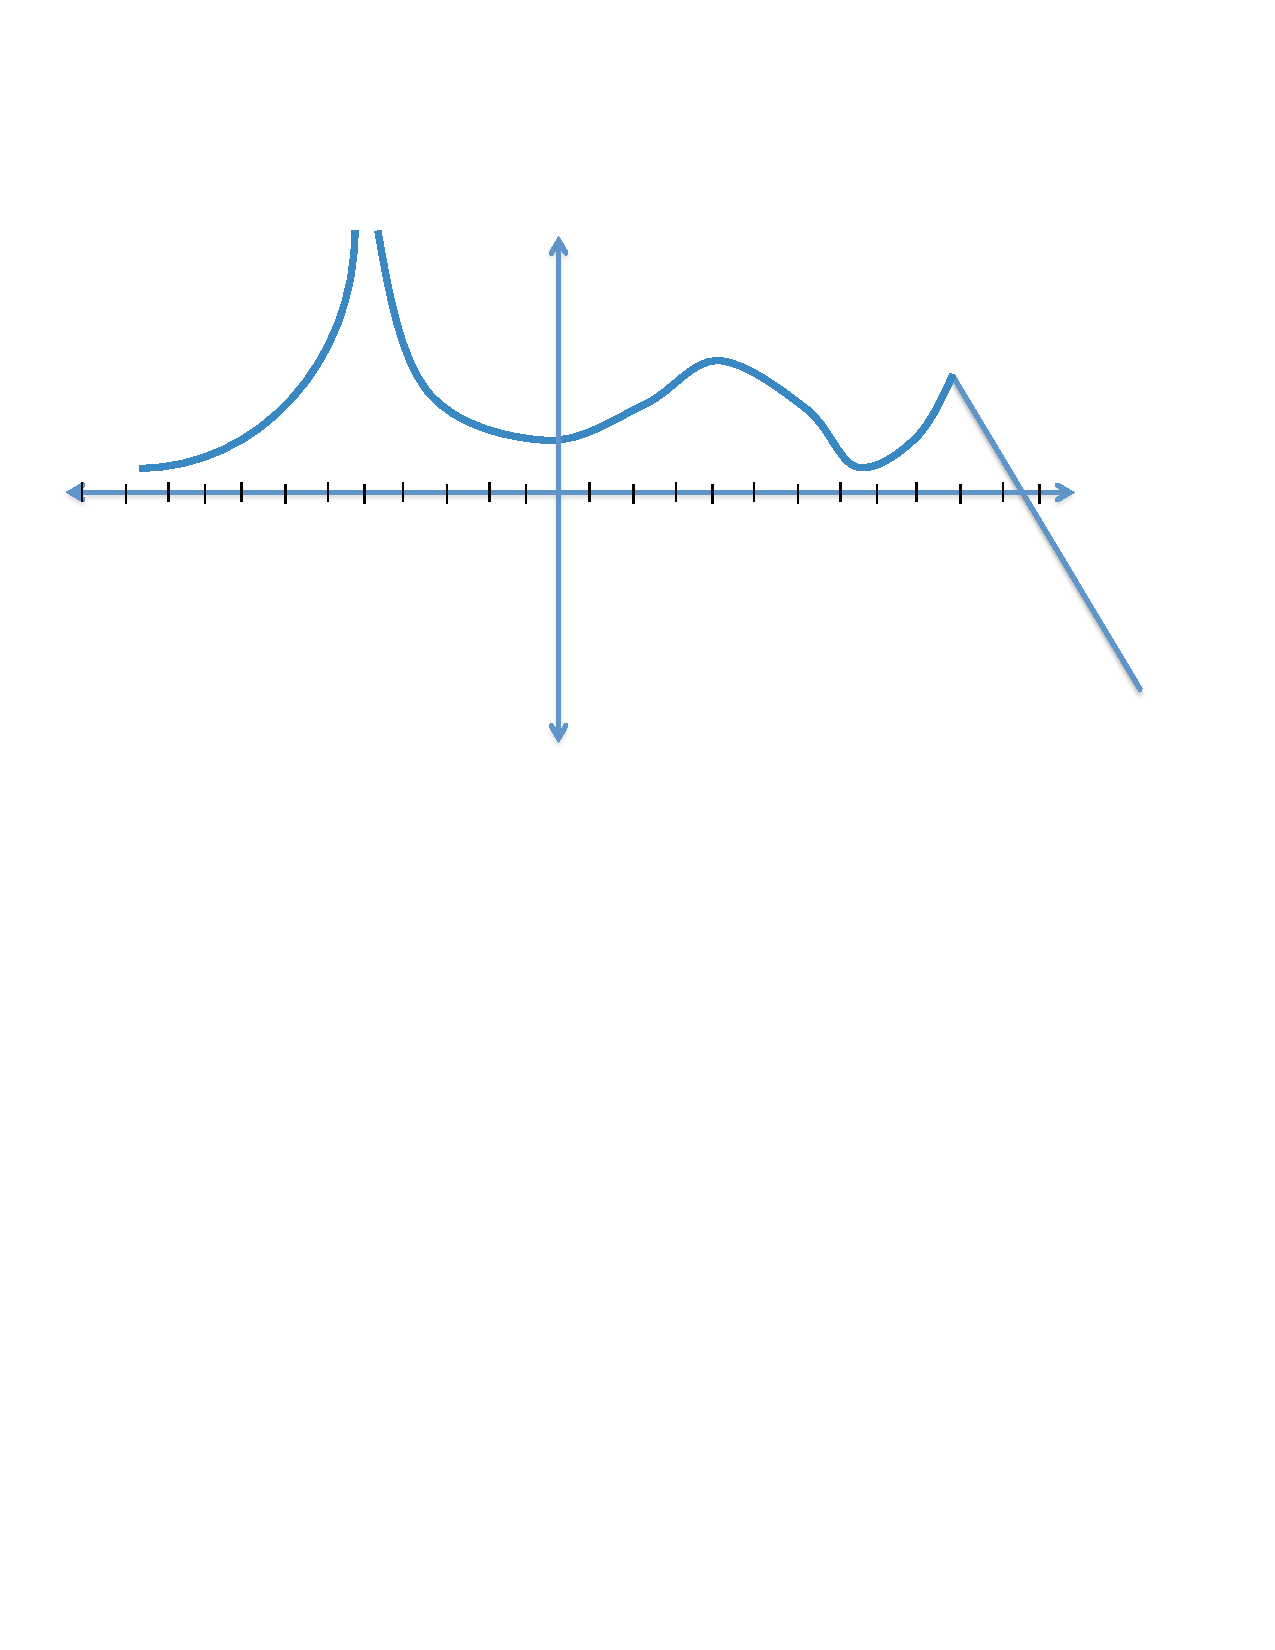
\includegraphics[scale=.5]{Figure5.pdf}
  \end{center}
	\end{freeResponse}
\end{enumerate}

\end{problem}

\end{document} 


















